\documentclass[10pt,a4paper]{report}  %紙張設定
\usepackage{xeCJK}%中文字體模組
\setCJKmainfont{標楷體} %設定中文字體
%\setCJKmainfont{MoeStandardKai.ttf}
\newfontfamily\sectionef{Times New Roman}%設定英文字體
%\newfontfamily\sectionef{Nimbus Roman}
\usepackage{enumerate}
\usepackage{amsmath,amssymb}%數學公式、符號
\usepackage{amsfonts} %數學簍空的英文字
\usepackage{graphicx}%圖形
\usepackage{caption,subcaption}
\usepackage{fontawesome5} %引用icon
\usepackage{type1cm} %調整字體絕對大小
\usepackage{textpos} %設定文字絕對位置
\usepackage{titlesec} %目錄標題設定模組
\usepackage{titletoc} %目錄內容設定模組
\usepackage{textcomp} %表格設定模組
\usepackage{multirow} %合併行
%\usepackage{multicol} %合併欄
\usepackage{CJK} %中文模組
\usepackage{CJKnumb} %中文數字模組
\usepackage{wallpaper} %浮水印
\usepackage{listings} %引用程式碼
\usepackage{hyperref} %引用url連結
\usepackage{setspace}
\usepackage{lscape}%設定橫式
%\lstset{language=Python, %設定語言
%basicstyle=\fontsize{10pt}{2pt}\selectfont, %設定程式內文字體大小
%frame=lines,	%設定程式框架為線
%}
\graphicspath{{./../images/}} %圖片預設讀取路徑
\usepackage{indentfirst} %設定開頭縮排模組
%\renewcommand{\figurename}{\Large 圖.} %更改圖片標題名稱
%\renewcommand{\tablename}{\Large 表.}
\renewcommand{\lstlistingname}{\Large 程式.} %設定程式標示名稱
%\hoffset=-5mm %調整左右邊界
%\voffset=-8mm %調整上下邊界
\setlength{\parindent}{2em}%設定首行行距縮排
%\usepackage{appendix} %附錄
\usepackage{diagbox}%引用表格
\usepackage{multirow}%表格置中
%======== 版 面 設 定 ========%
\usepackage[margin=2.5cm]{geometry}
%\setlength\columnsep{1cm}%調整雙欄位的中間間隔距離
%=------------------字型設定----------------------=%
\newfontfamily{\barial}{arialbd}%設定粗體Arial字體
[Extension = .ttf]
\newfontfamily{\timesbi}{timesbi}%設定粗斜體Times New Roman字體
[Extension = .ttf]
\newfontfamily{\timesbd}{timesbd}%設定粗體Times New Roman字體
[Extension = .ttf]
%=------------------圖標----------------------=%
\usepackage{subcaption}
%=------------------頁首----------------------=%
\usepackage{fancyhdr}%頁首頁尾
\pagestyle{fancy}
\renewcommand{\headrulewidth}{0pt}%去除頁首橫線
\fancyhead[R]{
\vspace{-5pt}\hspace{-1.3em} 
\fontsize{9pt}{2pt}\barial
Proceedings of 2021 International Conference on Mechatronic, Automobile, and Environment Engineering\\
October 22-24, 2021, Hualien, Taiwan\\[5pt]
Paper ID:xxxx}
%=-------------------------本文----------------------=%
\begin{document}
%=-------------------------標題----------------------=%
\begin{center}
\quad \\[1pt]
\fontsize{22pt}{3pt}\selectfont\hspace{0.35cm}\textbf{\sectionef Application of reinforcement learning in \\[12pt]
 mechatronic systems}\\[12pt]
\end{center}
%=-------------------------作者與聯繫方式----------------------=%
\begin{center}
\qquad \\[27pt]
First-Name Last-Name1, First-Name Last-Name2, First-Name Last-Name3\\[12pt]
1 Affiliation, E-mail:\\[6pt]
2 Affiliation, E-mail:\\[6pt]
3 Affiliation, E-mail:\\[6pt]
*Corresponding E-mail: \\
\qquad \\
\end{center}
%=-------------------------內容----------------------=%
\fontsize{10pt}{13pt}\selectfont
\begin{flushleft}
\timesbi Abstract:\sectionef 
近年來硬體技術、軟體、自動求導等技術快速發展起來,再次帶起機器學習的發展,促使機器學習與各領域結合的應用越來越廣泛,在機電系統採用強化學習是為了讓機電系統的控制達到最佳化。本研究利用強化學習優化冰球機的對打系統,並測試將相同的訓練算法能在2D環境上進行訓練和使用,將相同演算法套用到3D模擬環境進行訓練與使用,以驗證算法若將既有機電系統簡化成2D所測試的算法套用到3D模擬環境的可行性。將實體冰球機的機電系統簡化後導入CoppeliaSim模擬環境透過Remote API控制環境中的冰球機移動,OpenCV來處理影像提供強化學習訓練和訓練後實際控制的輸入,強化學習訓練利用OpenAI Gym的Pong Game測試適合的訓練參數,再將算法套用到CoppeliaSim的場景中進行訓練。\\%(須補結果、結論)
\end{flushleft}
\begin{flushleft}
\timesbi Keywords:\sectionef 類神經網路、強化學習、 CoppeliaSim、OpenAI Gym
\end{flushleft}
\vspace{1pt}
\begin{flushleft}
\fontsize{12pt}{12pt} \timesbd{Introduction}\\
\end{flushleft}

%介紹論文的範圍和目標並說明問題
由於機器學習的訓練需要透過長時間的訓練,測試合適的機器學習算法和參數需要長時間的測試與訓練才能得到適用的演算法,若以實體的機電系統進行訓練需要投入大量的金錢與時間成本,採取虛擬訓練的方式:在相同時間下可以訓練的次數較多實體環境中多,改善訓練時間冗長和組裝實體系統的成本。測試在2D環境中的演算法在3D環境下的可行性並評估演算法若套用到實體系統可行性。\\

相關文獻\\

%描述方法
透過OpenAI Gym內建編譯的Pong 遊戲環境當作2D的訓練環境,3D則是透過CoppeilaSim來模擬訓練機電系統的運作狀況,訓練演算法選用強化學習結合類神經網路的學習方式,其中使用score function gradient當作主要算法。\\

概述工作的主要結果\\

%本文目的是將相同的訓練算法能在2D環境上進行訓練和使用,將相同演算法套用到3D模擬環境進行訓練與使用,以驗證算法若將既有機電系統簡化成2D所測試的算法套用到3D模擬環境的可行性。將實體冰球機的機電系統簡化後導入CoppeliaSim模擬環境透過Remote API控制環境中的冰球機移動,OpenCV來處理影像提供強化學習訓練和訓練後實際控制的輸入,強化學習訓練利用OpenAI Gym的Pong Game測試適合的訓練參數,再將算法套用到CoppeliaSim的場景中進行訓練。\\
%近年來硬體技術、軟體、自動求導等技術快速發展起來,再次帶起機器學習的發展,促使機器學習與各領域結合的應用越來越廣泛,在機電系統採用強化學習是為了讓機電系統的控制達到最佳化。本研究利用強化學習優化冰球機的對打系統,並測試相同演算法運用在2D與3D模擬環境可行性。\\
%本研究分成兩大部分,第一部分簡化冰球機並運用OpenAI Gym的Atari Pong-v0測試較合適的訓練參數,在2D環境中進行強化學習的對打訓練。第二部分獎實體系統簡化後導入CoppeliaSim模擬環境導入測試完成的訓練參數進行虛擬訓練,進行算法導入到實體機前的測試。\\
\begin{figure}[hbt!]
\begin{center}
\subfigure{
\begin{minipage}[t]{0.3\linewidth}  %設定圖片間距
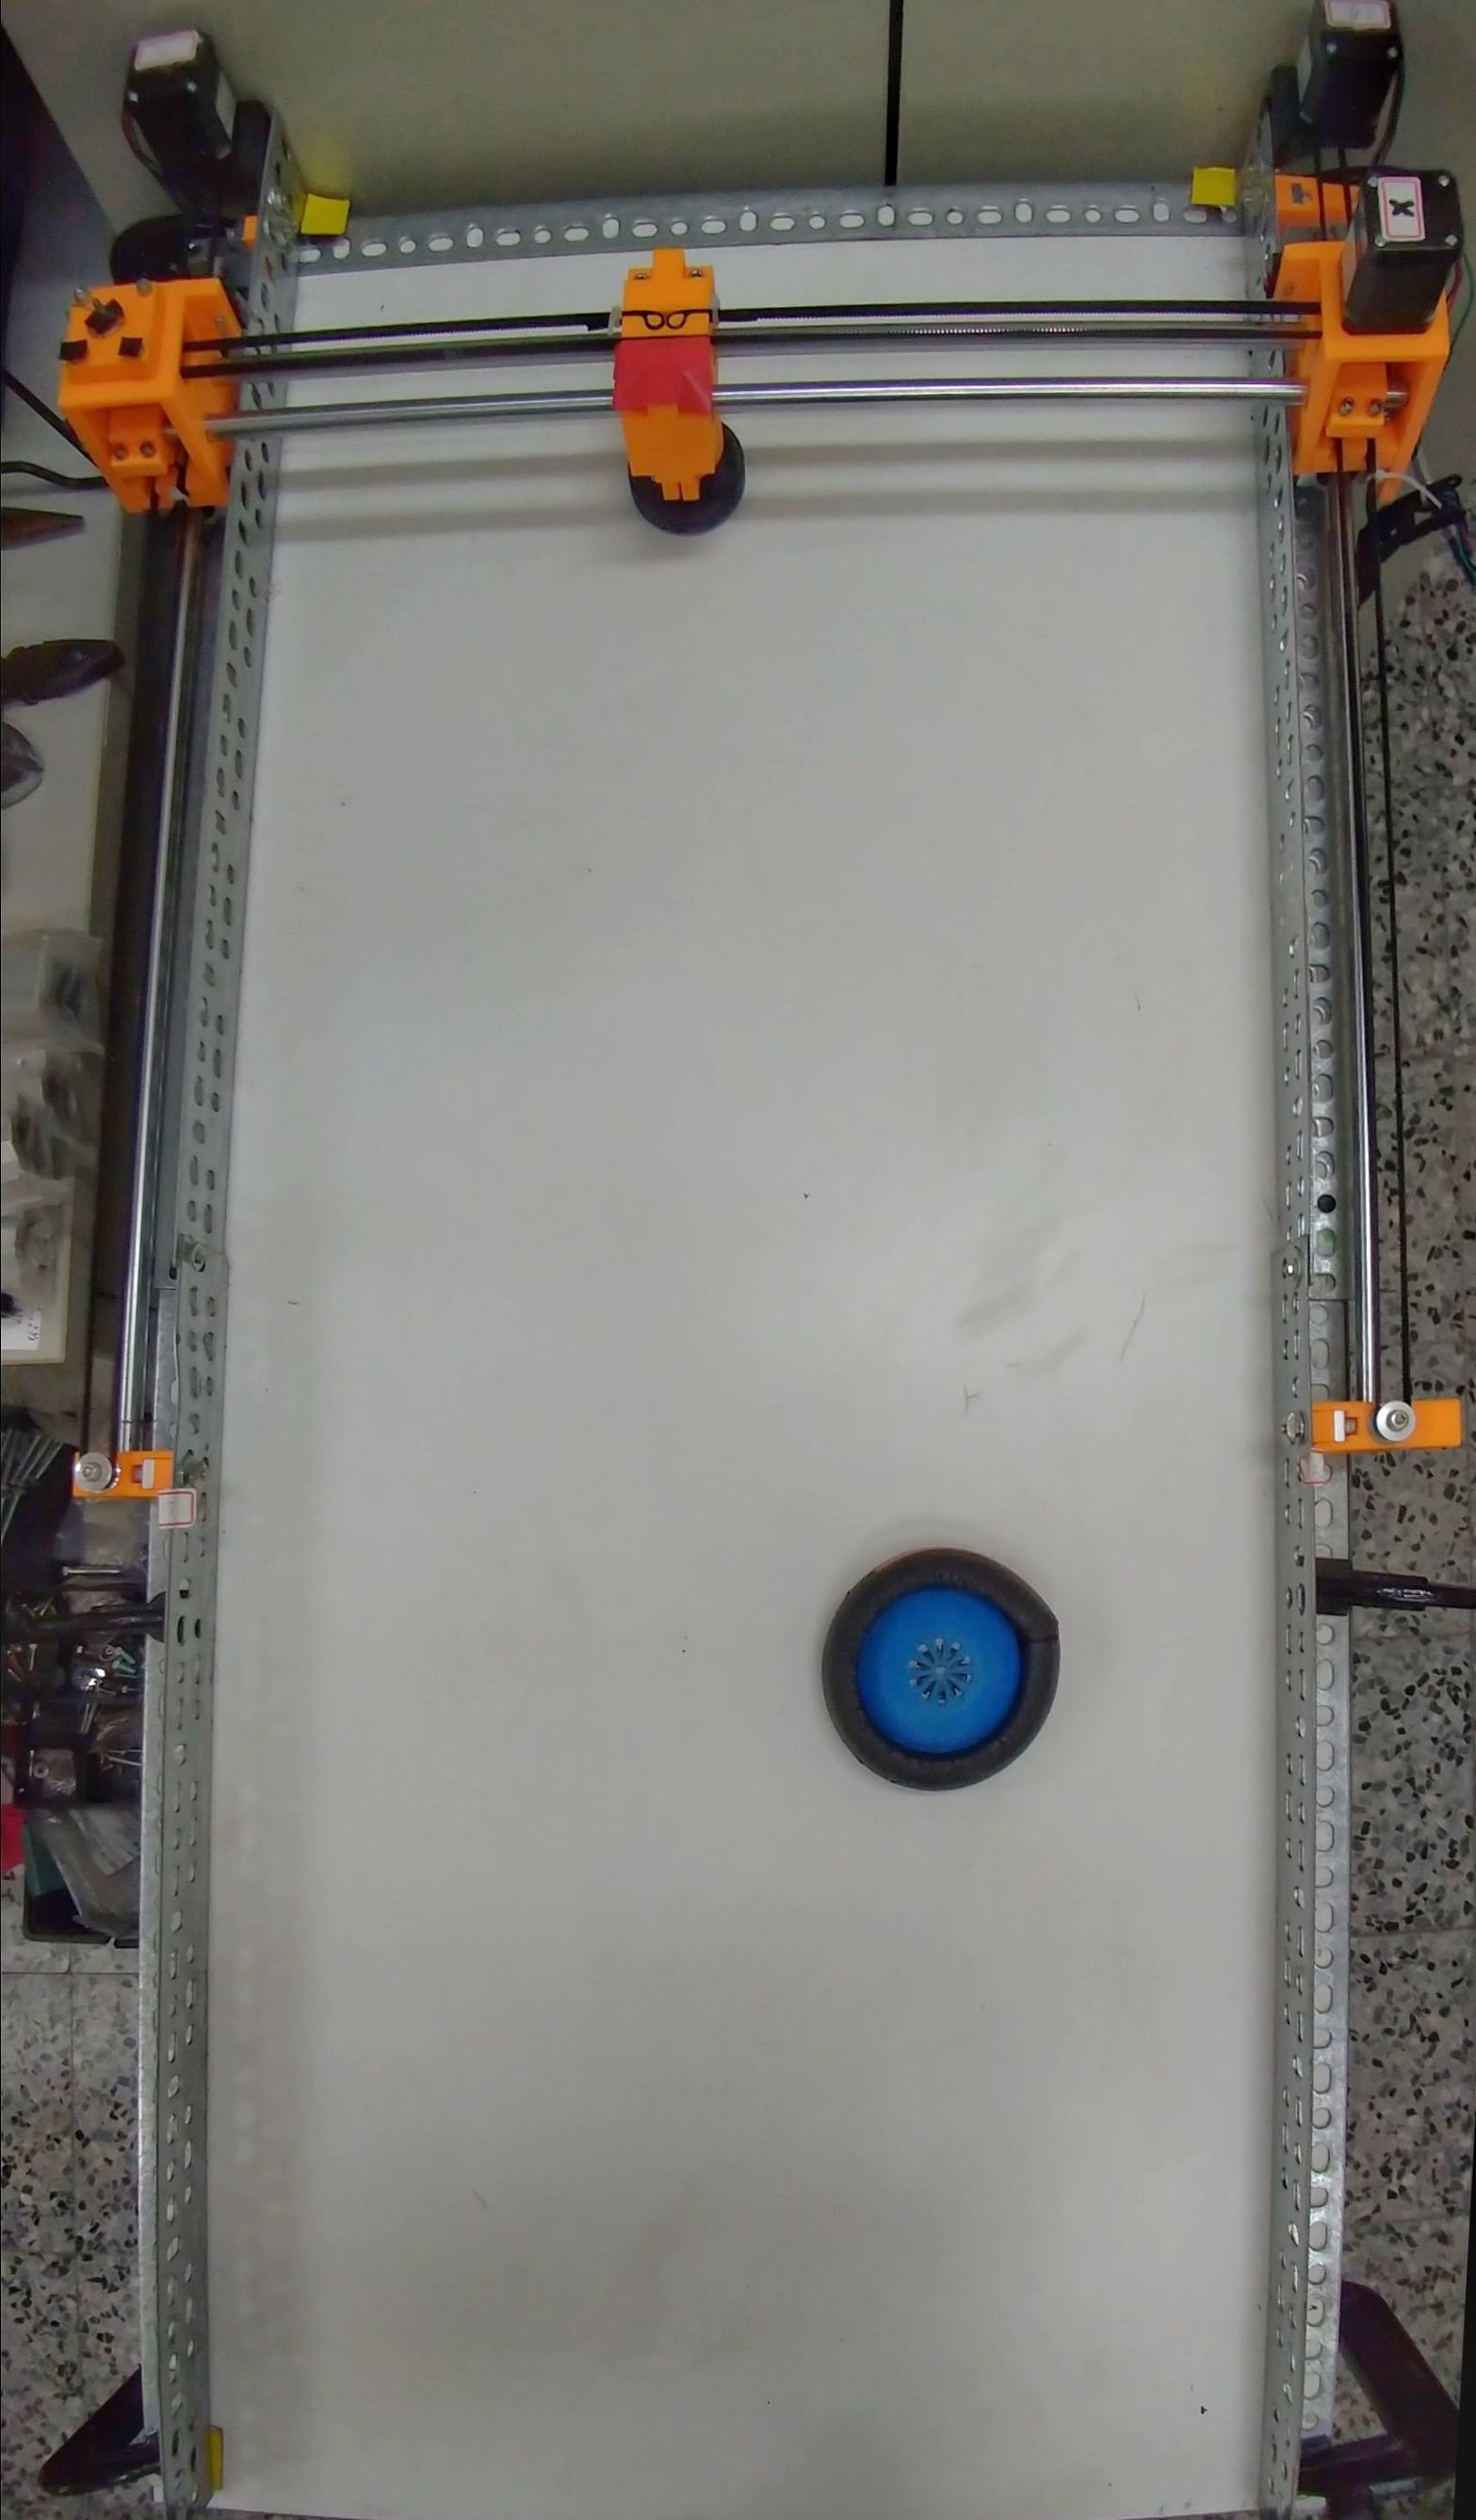
\includegraphics[width=4cm]{冰球機}
\caption{\Large 實體的冰球機}\label{fig.冰球機}
\end{minipage}
}
\subfigure{
\begin{minipage}[t]{0.3\linewidth}
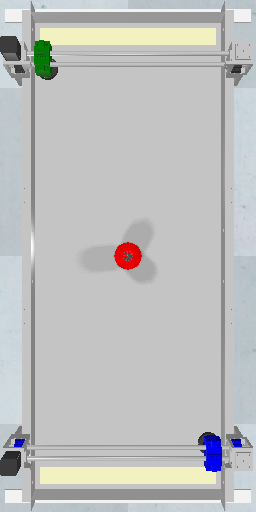
\includegraphics[width=4cm]{origin}
\caption{\Large 虛擬環境簡化後的冰球機}\label{fig.模擬冰球機}
\end{minipage}
}
\subfigure{
\begin{minipage}[t]{0.3\linewidth} 

\includegraphics[width=4cm]{pong_gym}
\caption{\Large Gym的Pong game}\label{fig.pong_gym}
\end{minipage}
}
\end{center}
\end{figure}
\newpage
\begin{flushleft}
{\large \timesbd{Methodology}}\\
\end{flushleft}

%方法論述
強化學習是環境和agent互動並互相影響著,以獎勵的方式鼓勵學習,並且不需要特別教導。類神經網路則是透過神經元之間的非線性與權重產生記憶性並學習,以back-propagation的方式修正權重與偏差達到進步的效果。結合類神經網路和強化學習這兩種算法,使訓練不需特別教導並以獎懲的方式鼓勵最大化得分,並在固定次數訓練後back-propagation修正權重偏差。\\

參考資料\\

解釋研究問題\\

描述研究框架\\
將對打系統的基本移動控制藉由強化學習來達到最佳化,透過Gym測試演算法可行性再進一步運用CoppeilaSim進行3D模擬環境訓練對打系統,後續可藉由冰球機結合網路攝影機將整個對打系統實際運用。

應用的方法\\

研究問題與理論和實踐相關\\

為什麼選擇的方法解決該問題\\

%藉由實體冰球機的零件透過Solidworks繪製、組立再導入虛擬環境
\begin{flushleft}
{\large \timesbd{Findings}}\\
\end{flushleft}
設計流程分為簡化模、型機器學習訓練、模擬環境訓練。\\
\textbf{簡化模型}
將冰球機簡化成一個自由度,簡化後與Pong的操控相同,並分別透過2D遊戲Pong-v0與3D模擬環境CoppilaSim供強化學習訓練。\\

\textbf{機器學習訓練}
透過影像處理,過濾出擊錘與球,並將兩幀影像進行比較,透過調整環境參數與決策參數的權重,環境參數使用ReLU Function進行優化,決策參數則是透過Log probability和Softmax進行運算並在每局結束後透過back-propgation修正與更新偏差,藉由不斷的學習持續進步。\\

\textbf{模擬環境訓練}
在CoppilaSim中,抓取場景中的攝影機,
\begin{flushleft}
{\large \timesbd{Conclusions}}\\
\end{flushleft}

推斷結果的原則和概括\\

工作的任何例外、問題或限制\\

工作的理論和或實踐意義\\

得出的結論和建議\\
\begin{flushleft}
{\large \timesbd{Acknowledgements}}\\
\end{flushleft}
\begin{flushleft}
{\large \timesbd{References}}\\
\end{flushleft}
%\input{test_reference.tex}
\end{document}